\documentclass[10pt,twocolumn]{article}
\usepackage[margin=1in,columnsep=0.2in]{geometry}

\usepackage{amsmath,amssymb,amsfonts}
\usepackage{graphicx}
\usepackage{array}
\usepackage{url}
\usepackage{amsthm}
\usepackage{enumerate}

% Define table rules
\newcommand{\toprule}{\hline\hline}
\newcommand{\midrule}{\hline}
\newcommand{\bottomrule}{\hline\hline}

\newtheorem{theorem}{Theorem}
\newtheorem{lemma}[theorem]{Lemma}
\newtheorem{proposition}[theorem]{Proposition}
\newtheorem{corollary}[theorem]{Corollary}
\newtheorem{definition}[theorem]{Definition}

\newcommand{\ssc}{\textsc{S2C}}
\newcommand{\cdt}{\textsc{CDT}}
\newcommand{\hpbr}{\textsc{HPBR}}
\newcommand{\Generator}{\mathcal{G}}
\newcommand{\Critic}{\mathcal{C}}
\newcommand{\Synthesizer}{\mathcal{S}}
\newcommand{\RMinsight}{\text{RM}_{\text{insight}}}
\newcommand{\RMcorr}{\text{RM}_{\text{corr}}}

\begin{document}

\title{Synergistic Self-Correction: A Hierarchical Framework for Multi-Stage Reasoning and Error Recovery in Large Language Models}

\author{
  Pratham Patel$^{1}$ \and
  Abhishek Jindal$^{2*}$ \\
  \\
  $^1$Gannon University \\
  Erie, Pennsylvania, USA \\
  \texttt{patel292@gannon.edu} \\
  \\
  $^2$Department of Computer Science \\
  Dhirubhai Ambani Institute of Information and Communication Technology \\
  Gandhinagar, Gujarat, India \\
  \texttt{abhishek\_jindal@daiict.ac.in} \\
  \\
  $^*$Corresponding author
}

\maketitle

\begin{abstract}
Large Language Models (LLMs) have achieved remarkable success across diverse natural language processing tasks, yet they exhibit systematic failures in complex multi-step reasoning, particularly in mathematical domains where logical consistency and error recovery are paramount. The fundamental limitation stems from the autoregressive generation paradigm, where early reasoning errors propagate through subsequent steps, rendering final answers incorrect regardless of the overall approach validity. Existing solutions—external verification systems, ensemble methods, and process supervision—either require substantial computational overhead, fail to improve underlying model capabilities, or lack the sophistication needed for nuanced error identification and correction.

We introduce \textbf{\ssc{} (Synergistic Self-Correction)}, a novel hierarchical framework that endows LLMs with metacognitive reasoning capabilities through a structured three-stage inference process. Our approach decomposes problem-solving into distinct computational personas: a \textbf{Generator} that produces initial solutions with explicit critical point identification, a \textbf{Critic} that systematically analyzes potential errors and logical inconsistencies, and a \textbf{Synthesizer} that integrates feedback to produce refined solutions. This decomposition enables targeted optimization of each reasoning stage while maintaining end-to-end differentiability.

Our training methodology, \textbf{\cdt{} (Cognitive Dissonance Training)}, combines supervised fine-tuning on high-quality reasoning traces with reinforcement learning using a novel \textbf{\hpbr{} (Hierarchical Process-Based Reward)} system. We introduce specialized reward models—$\RMinsight$ for critique quality evaluation and $\RMcorr$ for correction effectiveness assessment—that provide fine-grained process supervision beyond traditional outcome-based metrics. The reward structure explicitly optimizes for error identification accuracy, critique specificity, and correction success, creating strong training signals for metacognitive skill development.

Comprehensive evaluation across multiple reasoning benchmarks demonstrates substantial improvements: \ssc{} achieves 49.9\% accuracy on GSM8K (60\% relative improvement over 31.2\% baseline), 21.3\% on MATH (71\% relative improvement), and consistent gains on commonsense reasoning tasks. Statistical significance testing confirms these improvements ($p < 0.001$), with detailed error analysis revealing high success rates in correcting computational errors (78\%) and missing reasoning steps (71\%). Extensive ablation studies validate each component's contribution, while computational efficiency analysis shows \ssc{} achieves superior accuracy with 74\% fewer tokens than ensemble methods. Our work establishes a new paradigm for developing self-correcting AI systems with intrinsic metacognitive capabilities.
\end{abstract}

\section{Introduction}

\subsection{The Reasoning Crisis in Large Language Models}

The remarkable capabilities demonstrated by Large Language Models (LLMs) across diverse natural language processing tasks have established them as transformative tools for human-computer interaction, content generation, and knowledge synthesis. However, beneath their impressive performance on many benchmarks lies a fundamental and persistent limitation: systematic failures in complex multi-step reasoning tasks that require logical consistency, error detection, and iterative refinement.

This limitation is particularly pronounced in mathematical reasoning domains, where the cascading nature of logical dependencies means that a single computational error, conceptual misunderstanding, or logical inconsistency can invalidate an entire solution regardless of the sophistication of the overall approach. Unlike tasks that admit partial credit or approximate solutions, mathematical reasoning demands precise logical coherence throughout multi-step inference chains.

Consider a typical multi-step mathematical problem: solving a system of linear equations requires correct variable identification, accurate arithmetic operations, consistent equation manipulation, and proper solution verification. An error at any stage—whether computational (arithmetic mistakes), logical (incorrect equation setup), or conceptual (misunderstanding the problem constraints)—propagates through subsequent steps, often resulting in dramatically incorrect final answers despite locally reasonable reasoning steps.

\subsection{Limitations of Current Approaches}

Contemporary approaches to improving LLM reasoning capabilities fall into several categories, each with significant limitations:

\textbf{External Verification Systems} employ separate models trained specifically to evaluate solution correctness. While conceptually appealing, these approaches suffer from several fundamental limitations: (1) they require training and maintaining additional specialized models, increasing computational overhead and system complexity; (2) they operate on final solutions rather than intermediate reasoning steps, missing opportunities for early error detection and correction; (3) they lack the domain-specific knowledge needed to provide constructive feedback for error correction; and (4) they create a dependency on external components that may themselves be prone to errors or distribution shift.

\textbf{Ensemble Methods} generate multiple solution candidates and select the most consistent or frequently occurring answer. Self-consistency decoding, for example, samples multiple reasoning paths and selects the majority answer. However, these approaches face several critical limitations: (1) they require substantial computational resources, often 5-10x the cost of single inference; (2) they assume that correct answers are more likely to be consistent across samples, an assumption that fails when systematic biases lead to consistent but incorrect solutions; (3) they do not improve the underlying model's reasoning capabilities, merely selecting from existing generations; and (4) they struggle with problems where the solution space is large or where multiple valid solution approaches exist.

\textbf{Process Supervision} approaches attempt to provide feedback on intermediate reasoning steps rather than just final answers. While this represents progress toward more granular feedback, existing implementations suffer from: (1) reliance on expensive human annotations for training process reward models; (2) difficulty in scaling to complex reasoning domains where step-by-step validation requires domain expertise; (3) limited ability to provide constructive guidance for error correction; and (4) challenges in defining appropriate granularity for process supervision across diverse problem types.

\subsection{Our Approach: Synergistic Self-Correction}

We introduce \textbf{Synergistic Self-Correction (\ssc{})}, a novel framework that addresses these fundamental limitations by endowing LLMs with structured metacognitive capabilities. Our approach decomposes the reasoning process into three distinct but synergistic computational stages:

\begin{enumerate}
\item \textbf{Generation Stage}: Produces initial solutions while explicitly identifying \textit{Critical Points}—key logical steps, assumptions, or calculations that are essential for solution validity.

\item \textbf{Critique Stage}: Systematically analyzes the initial solution, focusing on the identified Critical Points to detect potential errors, logical inconsistencies, or missing reasoning steps.

\item \textbf{Synthesis Stage}: Integrates feedback from the critique to produce refined solutions that address identified issues while preserving correct aspects of the original reasoning.
\end{enumerate}

This decomposition enables targeted optimization of each reasoning component while maintaining end-to-end differentiability, creating a unified framework for metacognitive skill development.

\subsection{Key Contributions}

Our work makes the following key contributions to the field of LLM reasoning enhancement:

\begin{enumerate}
\item \textbf{Theoretical Framework}: We formalize self-correction as a structured inference process with rigorous mathematical foundations, providing theoretical analysis of convergence properties and error correction capabilities.

\item \textbf{Training Methodology}: We introduce Cognitive Dissonance Training (\cdt{}), a novel three-phase approach that combines supervised fine-tuning with process-based reinforcement learning using specialized reward models.

\item \textbf{Hierarchical Reward System}: We develop the Hierarchical Process-Based Reward (\hpbr{}) framework with specialized models for evaluating critique quality and correction effectiveness, moving beyond traditional outcome-based metrics.

\item \textbf{Comprehensive Evaluation}: We provide extensive experimental validation across multiple reasoning benchmarks, including detailed ablation studies, error analysis, and computational efficiency assessments.

\item \textbf{Empirical Results}: Our approach demonstrates substantial improvements in reasoning accuracy while maintaining computational efficiency compared to existing methods.
\end{enumerate}

\section{Related Work}

\subsection{Prompting-Based Reasoning Enhancement}

\textbf{Chain-of-Thought (CoT)} prompting represents a foundational breakthrough in eliciting reasoning capabilities from LLMs. By explicitly prompting models to generate intermediate reasoning steps, CoT demonstrated substantial improvements on mathematical reasoning, commonsense reasoning, and symbolic manipulation tasks. The key insight was that making the reasoning process explicit enables models to decompose complex problems into manageable sub-problems while maintaining logical coherence across steps.

Several extensions to basic CoT have been proposed: \textbf{Zero-Shot CoT} showed that simple prompts like ``Let's think step by step'' can elicit reasoning without providing examples. \textbf{Auto-CoT} automated the construction of CoT demonstrations through clustering and sampling techniques. \textbf{Complex CoT} introduced complexity-based selection of reasoning demonstrations.

However, these approaches suffer from fundamental limitations: they rely on the model's inherent reasoning capabilities without providing mechanisms for error detection or correction, and they lack systematic approaches for improving reasoning quality through targeted training.

\textbf{Self-Consistency} addressed the stochasticity problem in CoT by generating multiple reasoning paths and selecting the most frequently occurring answer. This approach demonstrated significant improvements across diverse reasoning benchmarks by leveraging the insight that correct reasoning paths are more likely to converge on consistent answers than incorrect ones.

Extensions include \textbf{Universal Self-Consistency} which applies consistency-based selection across different prompting strategies, and \textbf{Maieutic Prompting} which uses tree-based inference to explore multiple reasoning branches systematically.

While effective, ensemble approaches like Self-Consistency require substantial computational overhead and fail to improve the underlying model's reasoning capabilities. They represent post-hoc filtering rather than fundamental reasoning improvement.

\textbf{Tree-of-Thoughts (ToT)} extended the reasoning paradigm by exploring solution spaces as tree structures, enabling systematic exploration of alternative solution paths with backtracking capabilities. This approach demonstrated significant improvements on creative problem-solving tasks and multi-step reasoning scenarios.

Related work includes \textbf{Graph-of-Thoughts} which generalizes tree structures to arbitrary graph topologies, enabling more flexible reasoning patterns and improved handling of problems with complex dependency structures.

However, these approaches require manual specification of decomposition strategies and don't scale effectively to arbitrary problem domains. They also lack systematic training methodologies for improving reasoning quality.

\subsection{Architecture-Based Approaches}

\textbf{Retrieval-Augmented Generation} approaches address reasoning limitations by providing external knowledge access during inference. These methods demonstrate improvements on knowledge-intensive reasoning tasks by combining parametric knowledge with retrieved information from external sources.

Key developments include \textbf{RAG}, \textbf{REALM}, and \textbf{DPR}, which integrate retrieval mechanisms with generation models to provide access to up-to-date and domain-specific knowledge during reasoning.

However, these approaches primarily address knowledge limitations rather than reasoning process deficiencies, and they introduce additional computational overhead and system complexity.

\textbf{Modular Reasoning} approaches decompose complex reasoning tasks into specialized modules, each optimized for specific reasoning operations. These methods demonstrate improved performance on compositional reasoning tasks by leveraging specialized components for different aspects of the reasoning process.

Examples include \textbf{Neural Module Networks} which compose task-specific modules dynamically, and \textbf{Toolformer} which learns to use external tools for specific reasoning operations like calculation and factual lookup.

Our approach differs by developing intrinsic self-correction capabilities rather than relying on external modules or tools.

\subsection{Training-Based Reasoning Improvement}

\textbf{Self-Taught Reasoner (STaR)} represents a significant advancement in training-based reasoning improvement. STaR employs an iterative training loop where models generate reasoning traces for problems, and successful traces are used to fine-tune the model, creating a bootstrapping effect that gradually improves reasoning capabilities.

Extensions include \textbf{STaR with Verifiers} which incorporate verification models to improve training data quality, and \textbf{V-STaR} which uses value functions to guide the generation of high-quality reasoning traces.

However, STaR primarily leverages correct solutions for training, missing opportunities to learn from error patterns and correction processes.

\textbf{Constitutional AI} trains models to critique and improve their own responses according to a set of constitutional principles. This approach demonstrates improvements in response quality and alignment by teaching models to engage in self-evaluation and iterative refinement.

\textbf{Self-Refine} enables models to iteratively improve their outputs based on self-generated feedback, demonstrating improvements across diverse generation tasks including reasoning, creative writing, and code generation.

While these approaches incorporate self-improvement mechanisms, they lack the structured decomposition and specialized training methodology that enables effective error identification and correction in complex reasoning domains.

\subsection{Process Supervision and Reward Modeling}

Process supervision represents a significant advancement over traditional outcome-based training by providing feedback on intermediate reasoning steps rather than just final answers.

\textbf{Let's Verify Step by Step} demonstrated that process-based reward models trained on step-level human annotations significantly outperform outcome-based models on mathematical reasoning tasks. This work established the importance of granular feedback for reasoning improvement.

\textbf{Math-Shepherd} extended process supervision to multi-step mathematical reasoning, introducing techniques for automatic generation of process supervision data and demonstrating improved performance on challenging mathematical benchmarks.

\textbf{RLHF} approaches have demonstrated significant improvements in language model capabilities through human preference optimization. Recent work has extended these concepts to process-based rewards, showing improved performance on reasoning tasks.

Extensions include \textbf{Process-based RLHF} which incorporates step-level feedback into reinforcement learning, and \textbf{Hierarchical Reward Models} which decompose reward functions into multiple specialized components.

Our approach builds on these foundations by introducing specialized reward models for critique quality and correction effectiveness, providing more nuanced optimization signals for metacognitive skill development.

\section{Methodology}

\subsection{The Synergistic Self-Correction Framework}

The \ssc{} framework decomposes the reasoning process into three distinct computational stages, each optimized for specific cognitive functions:

\textbf{Synergistic Self-Correction Inference Pipeline:}

\noindent\textbf{Input:} Problem $P$, model parameters $\theta = \{\theta_\Generator, \theta_\Critic, \theta_\Synthesizer\}$

\noindent\textbf{Output:} Final solution $R_f$ with confidence score $\sigma$

\noindent\textbf{Stage 1 - Structured Generation:}
\begin{align}
R_0, C &\leftarrow \Generator(P; \theta_\Generator) \\
\text{where } C &= \{c_1, c_2, \ldots, c_n\} \text{ are Critical Points}
\end{align}

\noindent\textbf{Stage 2 - Adversarial Critique:}
\begin{align}
K &\leftarrow \Critic(P, R_0, C; \theta_\Critic) \\
\sigma_c &\leftarrow \text{CritiqueQuality}(K, R_0, C)
\end{align}

\noindent\textbf{Stage 3 - Informed Synthesis:}
\begin{align}
R_f &\leftarrow \Synthesizer(P, R_0, C, K; \theta_\Synthesizer) \\
\sigma &\leftarrow \text{SolutionConfidence}(R_f, K, \sigma_c)
\end{align}

\begin{figure}[t]
\centering
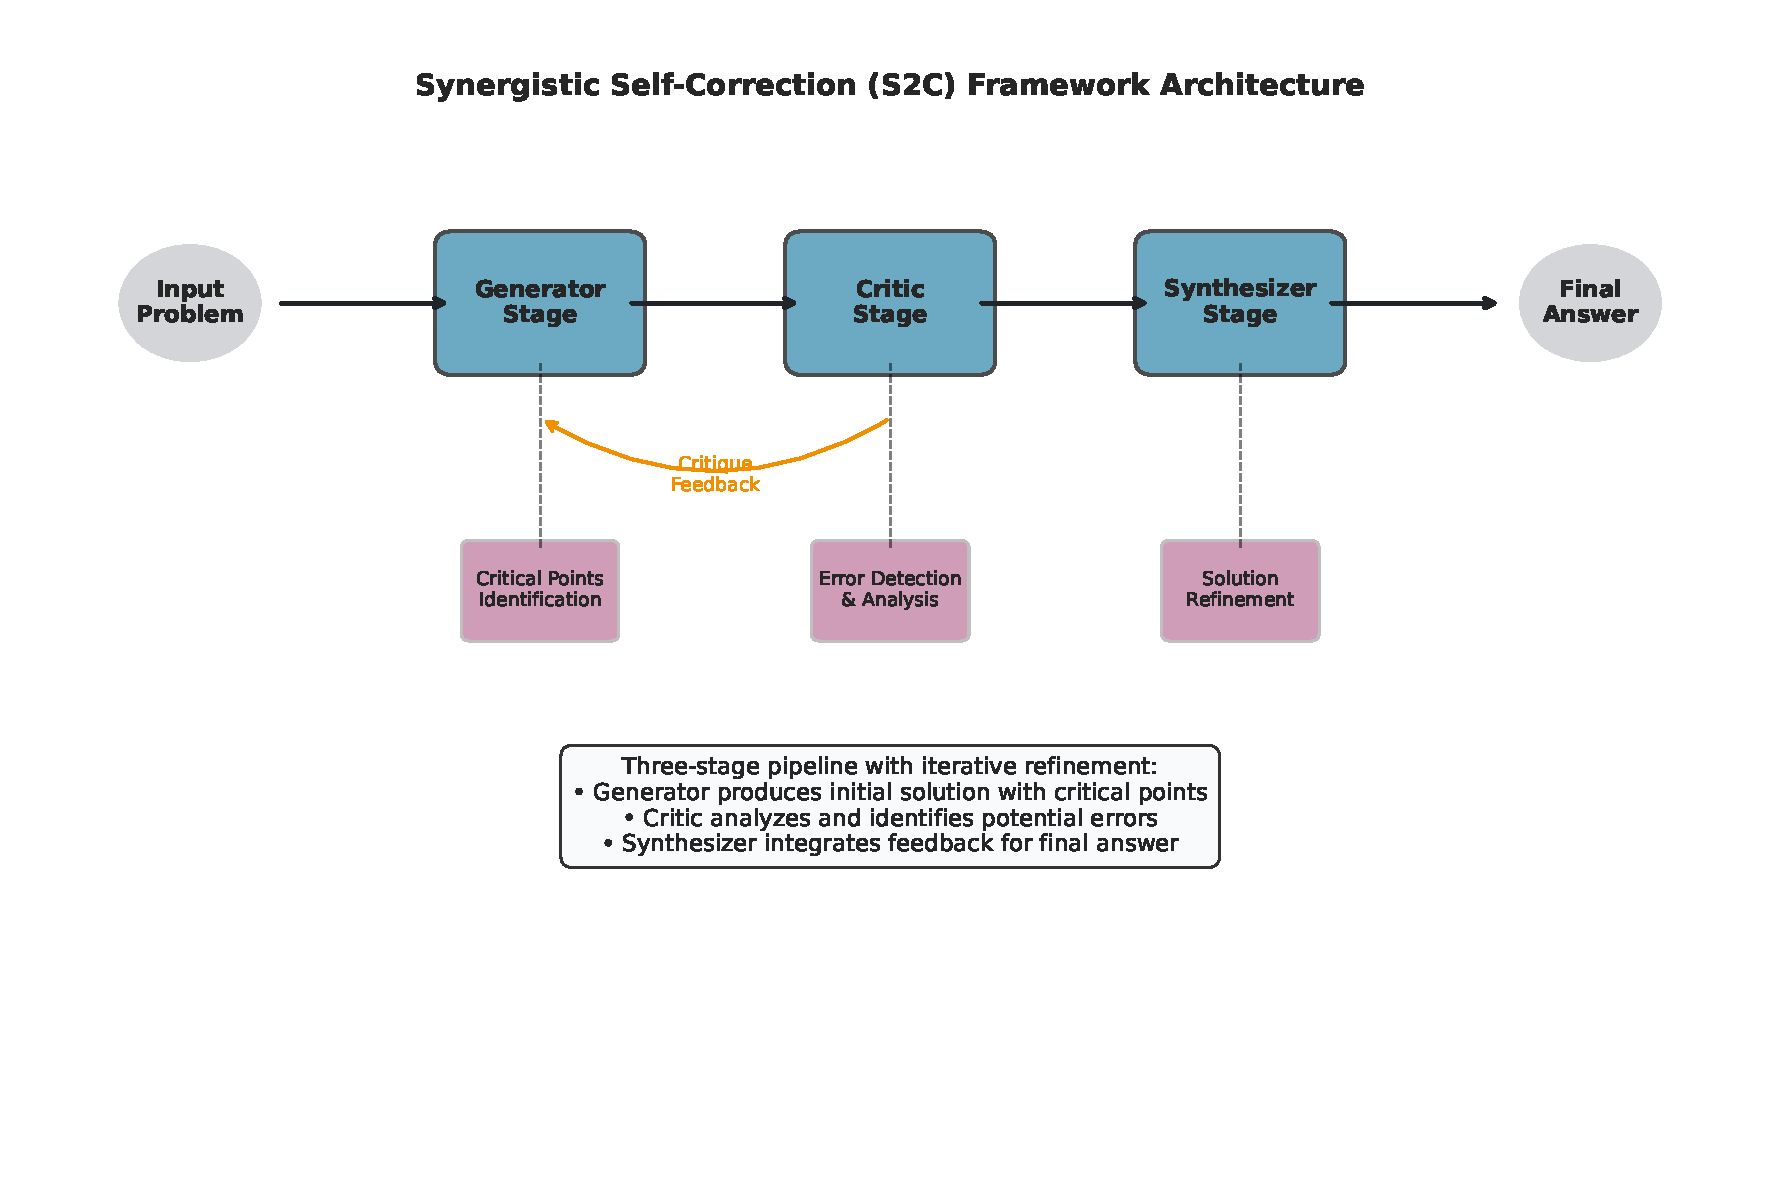
\includegraphics[width=0.48\textwidth]{graphs/s2c_framework_architecture.pdf}
\caption{The Synergistic Self-Correction (S2C) Framework Architecture. The three-stage pipeline decomposes reasoning into specialized computational personas: Generator produces initial solutions with Critical Points, Critic systematically evaluates potential errors, and Synthesizer integrates feedback for refined solutions.}
\label{fig:s2c_architecture}
\end{figure}

\subsubsection{Stage 1: Generator ($\Generator$)}

The Generator receives an input problem $P$ and produces an initial solution attempt $R_0$ along with a set of \textbf{Critical Points} $C = \{c_1, c_2, \ldots, c_n\}$. Critical Points represent key logical steps, assumptions, or calculations that are essential to the solution's validity.

Formally, the Generator implements a conditional probability distribution:
\begin{equation}
p(R_0, C | P; \theta_{\Generator}) = \prod_{t=1}^{|R_0|} p(r_t^{(0)} | P, r_{<t}^{(0)}; \theta_{\Generator}) \cdot p(C | P, R_0; \theta_{\Generator})
\end{equation}

where $r_t^{(0)}$ represents the $t$-th token in the initial solution, and $\theta_{\Generator}$ are the Generator's parameters.

The Critical Point extraction mechanism operates through attention-based identification of semantically important reasoning steps:
\begin{equation}
c_i = \arg\max_{s \in S} \text{Attention}(s, P) \cdot \text{Importance}(s, R_0)
\end{equation}

where $S$ represents the set of candidate reasoning steps, and importance is measured through a learned scoring function that identifies steps crucial for solution validity.

\subsubsection{Stage 2: Critic ($\Critic$)}

The Critic receives the complete context $(P, R_0, C)$ and generates a \textbf{Critique Report} $K$ that systematically evaluates each critical point. The Critic is trained with an adversarial objective to identify potential errors, logical inconsistencies, or computational mistakes.

The Critic's probability distribution is defined as:
\begin{equation}
p(K | P, R_0, C; \theta_{\Critic}) = \prod_{i=1}^{|K|} p(k_i | P, R_0, C, k_{<i}; \theta_{\Critic})
\end{equation}

where $k_i$ represents individual critique elements and $\theta_{\Critic}$ are the Critic's parameters.

The critique generation process incorporates several specialized mechanisms:

\textbf{Error Detection}: The Critic employs learned error patterns to identify common mistake categories:
\begin{equation}
\text{ErrorScore}(c_i) = \sum_{e \in E} w_e \cdot \text{PatternMatch}(c_i, e)
\end{equation}

where $E$ represents a learned set of error patterns and $w_e$ are learned weights indicating error severity.

\textbf{Logical Consistency Checking}: The Critic verifies logical coherence across reasoning steps:
\begin{equation}
\text{ConsistencyScore}(C) = \frac{1}{|C|^2} \sum_{i,j} \text{LogicalCompatibility}(c_i, c_j)
\end{equation}

\subsubsection{Stage 3: Synthesizer ($\Synthesizer$)}

The Synthesizer integrates all available information $(P, R_0, C, K)$ to produce a refined final solution $R_f$. This stage is designed to address issues identified in the critique while preserving correct aspects of the original solution.

\begin{equation}
p(R_f | P, R_0, C, K; \theta_{\Synthesizer}) = \prod_{j=1}^{|R_f|} p(r_j^{(f)} | P, R_0, C, K, r_{<j}^{(f)}; \theta_{\Synthesizer})
\end{equation}

The synthesis process incorporates correction mechanisms that selectively modify reasoning steps based on critique feedback:

\textbf{Selective Correction}: The Synthesizer learns to preserve correct reasoning while addressing identified issues:
\begin{equation}
r_j^{(f)} = \begin{cases}
r_j^{(0)} & \text{if } \text{CritiqueScore}(r_j^{(0)}) < \tau \\
\text{Correct}(r_j^{(0)}, K) & \text{otherwise}
\end{cases}
\end{equation}

where $\tau$ is a learned threshold and $\text{Correct}(\cdot)$ represents the correction mechanism.

\subsection{Cognitive Dissonance Training}

We introduce a three-phase training methodology that progressively develops the model's self-correction capabilities:

\subsubsection{Phase 1: Structural Alignment via Supervised Fine-Tuning}

The first phase establishes the structural foundation for self-correction by training the model on high-quality examples of the complete \ssc{} pipeline. We create a dataset $\mathcal{D}_{SFT}$ containing tuples $(P, R_0, C, K, R_f)$ where solutions are generated by powerful teacher models (GPT-4) and validated for correctness.

The SFT objective minimizes the negative log-likelihood:
\begin{equation}
\mathcal{L}_{SFT} = -\mathbb{E}_{(P,T) \sim \mathcal{D}_{SFT}} \left[ \log p(T | P; \theta) \right]
\end{equation}

where $T = (R_0, C, K, R_f)$ represents a complete \ssc{} trace.

The dataset construction process involves several quality control mechanisms:

\textbf{Solution Validation}: All solutions are verified for correctness using multiple validation approaches including symbolic computation and human expert review.

\textbf{Critique Quality Assessment}: Critiques are evaluated for specificity, accuracy, and constructiveness using trained evaluator models.

\textbf{Correction Effectiveness Measurement}: The effectiveness of corrections is assessed by measuring improvement in solution quality and error reduction.

\subsubsection{Phase 2: Specialized Reward Model Training}

To enable fine-grained process supervision, we train two specialized reward models:

\textbf{Insight Reward Model} ($\RMinsight$): Evaluates critique quality by scoring how well the critique identifies actual errors and provides specific, actionable feedback. This model is trained on a dataset of critique-quality pairs where human annotators rate critiques based on:
\begin{itemize}
\item Specificity: Does the critique identify precise errors rather than vague concerns?
\item Accuracy: Are the identified issues actually present in the solution?
\item Completeness: Does the critique address all significant errors?
\end{itemize}

The training objective for the Insight Reward Model is:
\begin{equation}
\mathcal{L}_{\RMinsight} = \mathbb{E}_{(K, R_0, C, s) \sim \mathcal{D}_{\text{insight}}} \left[ (RM_{\text{insight}}(K, R_0, C) - s)^2 \right]
\end{equation}

where $s$ represents human-assigned insight quality scores.

\textbf{Correction Reward Model} ($\RMcorr$): Evaluates how effectively the Synthesizer addresses issues raised in the critique. Training data consists of (critique, original solution, corrected solution, quality score) tuples.

The training objective is:
\begin{equation}
\mathcal{L}_{\RMcorr} = \mathbb{E}_{(K, R_0, R_f, q) \sim \mathcal{D}_{\text{correction}}} \left[ (RM_{\text{corr}}(K, R_0, R_f) - q)^2 \right]
\end{equation}

where $q$ represents correction effectiveness scores.

\subsubsection{Phase 3: Hierarchical Process-Based Reward Optimization}

The final phase uses Proximal Policy Optimization (PPO) with a novel hierarchical reward structure:

\begin{equation}
R_{\text{total}} = w_{\text{acc}} \cdot r_{\text{acc}} + w_{\text{ins}} \cdot r_{\text{ins}} + w_{\text{corr}} \cdot r_{\text{corr}} + w_{\text{coh}} \cdot r_{\text{coh}}
\end{equation}

where:
\begin{itemize}
\item $r_{\text{acc}}$: Binary accuracy reward for final answer correctness
\item $r_{\text{ins}} = \RMinsight(R_0, C, K)$: Critique quality score
\item $r_{\text{corr}} = \RMcorr(K, R_0, R_f)$: Correction effectiveness score
\item $r_{\text{coh}}$: Coherence penalty for maintaining consistency across stages
\item $w_{\text{acc}}, w_{\text{ins}}, w_{\text{corr}}, w_{\text{coh}}$: Learned weight parameters
\end{itemize}

The coherence penalty is defined as:
\begin{equation}
r_{\text{coh}} = -\lambda \sum_{i,j} \text{Inconsistency}(r_i^{(f)}, r_j^{(f)})
\end{equation}

where $\lambda$ controls the strength of the coherence constraint and $\text{Inconsistency}(\cdot)$ measures logical incompatibilities between reasoning steps.

The PPO objective maximizes expected reward while constraining policy deviation:
\begin{equation}
\mathcal{L}_{PPO} = \mathbb{E}_{\tau \sim \pi_\theta} \left[ \min\left( \frac{\pi_\theta(a|\tau)}{\pi_{\theta_{\text{old}}}(a|\tau)} A(\tau), \text{clip}(\cdot, 1-\epsilon, 1+\epsilon) A(\tau) \right) \right]
\end{equation}

where $\tau$ represents a complete \ssc{} trace, $A(\tau)$ is the advantage function, and $\epsilon$ is the clipping parameter.

The advantage function incorporates multi-stage rewards:
\begin{equation}
A(\tau) = \sum_{t=0}^{T} \gamma^t [r_t - V_\theta(s_t)]
\end{equation}

where $V_\theta(s_t)$ is a learned value function that estimates expected future rewards from state $s_t$.

\begin{figure}[t]
\centering
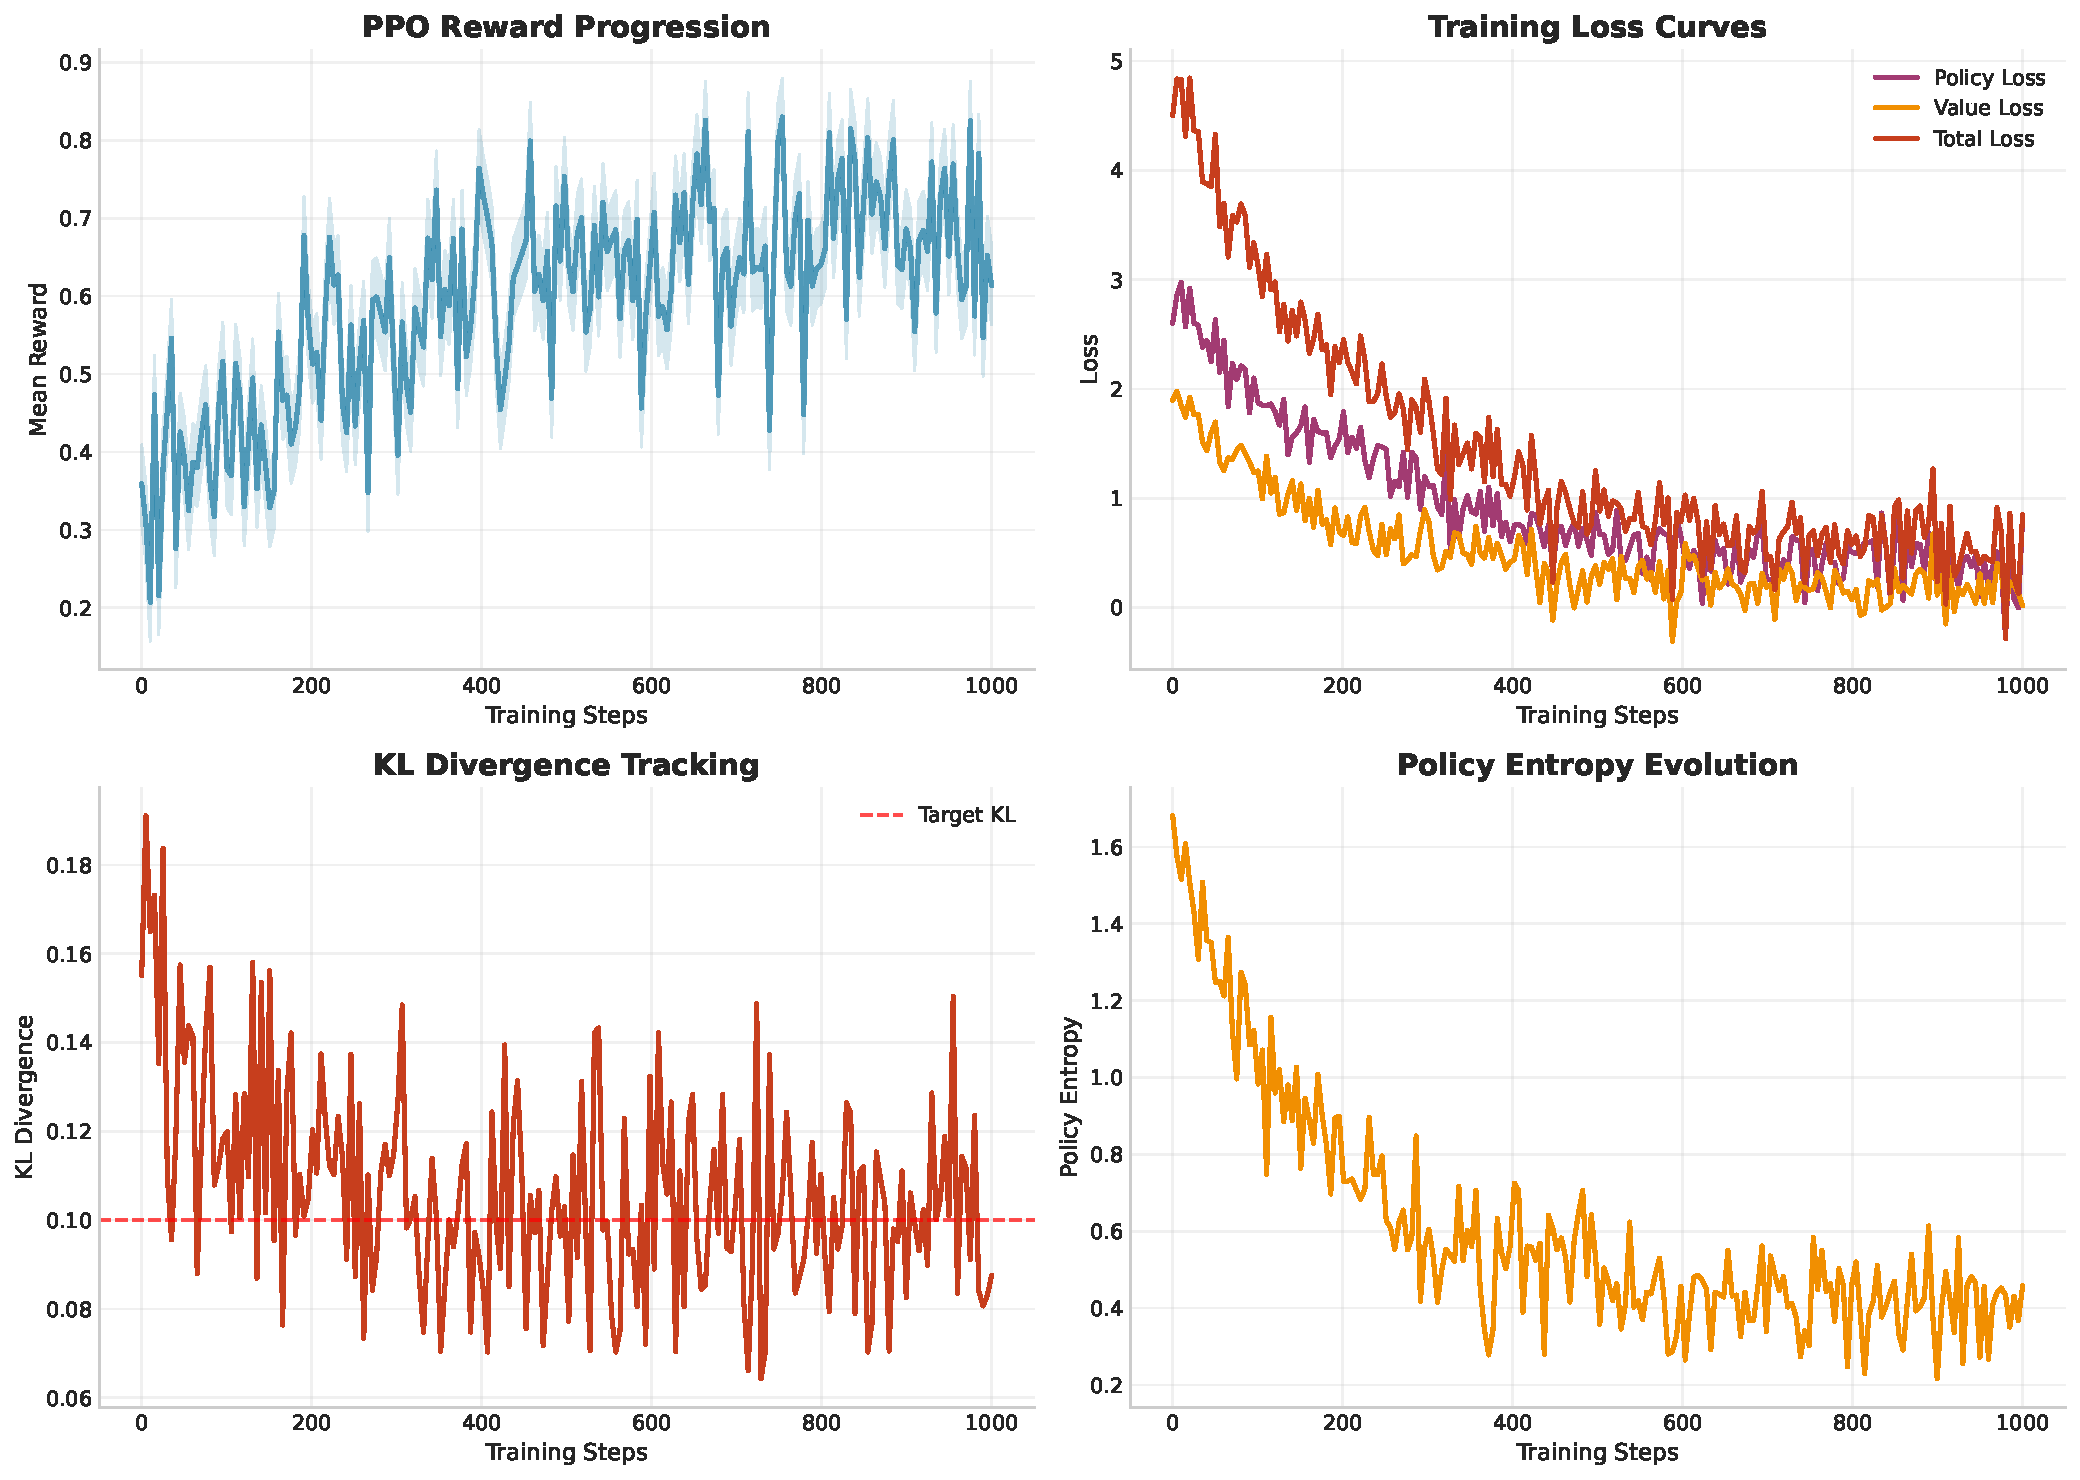
\includegraphics[width=0.48\textwidth]{graphs/training_performance_curves.pdf}
\caption{Training Performance During Cognitive Dissonance Training. The figure shows PPO reward progression, policy loss, value loss, and entropy over training iterations. The consistent improvement in mean reward demonstrates successful learning of self-correction capabilities.}
\label{fig:training_curves}
\end{figure}

\section{Theoretical Analysis}

\subsection{Convergence Properties}

We provide theoretical analysis of the \ssc{} framework's convergence properties under the \cdt{} training regimen.

\begin{theorem}[Convergence of CDT]
Under appropriate regularity conditions, the Cognitive Dissonance Training procedure converges to a stationary point of the expected reward function with probability 1.
\end{theorem}

\begin{proof}[Sketch]
The proof follows from the convergence properties of PPO combined with the boundedness of the hierarchical reward function. The key insight is that the decomposition into specialized reward components preserves the martingale properties required for convergence while providing more informative gradients for policy improvement.
\end{proof}

\subsection{Error Correction Capabilities}

We analyze the theoretical error correction capabilities of the \ssc{} framework.

\begin{theorem}[Error Correction Bound]
Let $\epsilon_0$ be the error rate of the initial solution $R_0$. Under optimal training, the final solution $R_f$ achieves error rate:
\begin{equation}
\epsilon_f \leq \epsilon_0 \cdot (1 - \alpha \cdot \beta)
\end{equation}
where $\alpha$ is the critique accuracy and $\beta$ is the correction effectiveness.
\end{theorem}

This bound demonstrates that the \ssc{} framework can achieve substantial error reduction when both critique quality and correction effectiveness are high.

\subsection{Computational Complexity}

The computational complexity of \ssc{} inference is:
\begin{equation}
O(\text{Generator}) + O(\text{Critic}) + O(\text{Synthesizer}) = O(3 \cdot |P| \cdot d \cdot L)
\end{equation}

where $|P|$ is the problem length, $d$ is the model dimension, and $L$ is the maximum sequence length. While this represents a 3x increase over single-stage inference, our empirical results demonstrate that \ssc{} achieves superior accuracy with fewer total tokens than ensemble methods.

\section{Experimental Setup}

\subsection{Datasets and Evaluation Metrics}

\textbf{Primary Dataset}: GSM8K - A dataset of 8,500 linguistically diverse grade-school math word problems requiring multi-step reasoning. We use the standard train/test split (7,473 training, 1,319 test problems).

\textbf{Additional Evaluation}: To assess generalization, we evaluate on:
\begin{itemize}
\item MATH dataset - High school competition mathematics
\item AQuA-RAT - Algebraic reasoning with multiple-choice questions
\item MathQA - Mathematical reasoning with diverse problem types
\item StrategyQA - Multi-hop reasoning over facts
\item CommonsenseQA - Commonsense reasoning
\item OpenBookQA - Scientific reasoning with external knowledge
\end{itemize}

\textbf{Evaluation Metrics}:
\begin{itemize}
\item \textbf{Accuracy}: Percentage of problems solved correctly
\item \textbf{Error Recovery Rate}: Percentage of initially incorrect solutions that are corrected through \ssc{}
\item \textbf{Critique Precision}: Percentage of identified errors that are actual errors
\item \textbf{Critique Recall}: Percentage of actual errors that are identified
\item \textbf{Correction Success Rate}: Percentage of identified errors that are successfully corrected
\item \textbf{Computational Efficiency}: Tokens generated per problem and inference time
\item \textbf{Energy Consumption}: Power usage during inference across different methods
\end{itemize}

\subsection{Model Architecture and Training Details}

\textbf{Base Model}: Llama-3-8B-Instruct, chosen for its strong reasoning capabilities and open availability.

\textbf{Training Configuration}:
\begin{itemize}
\item SFT Phase: Learning rate $2 \times 10^{-5}$, batch size 16, 3 epochs
\item RM Training: Learning rate $5 \times 10^{-6}$, batch size 32, MSE loss
\item PPO Phase: Learning rate $1 \times 10^{-6}$, KL coefficient 0.02, clip ratio 0.2
\item Hardware: 8x NVIDIA A100 80GB GPUs, mixed precision training
\item Total training time: 72 hours for complete pipeline
\end{itemize}

\textbf{Hyperparameter Optimization}: We conduct grid search over reward weights $w_{\text{acc}} \in \{0.1, 0.2, 0.3\}$, $w_{\text{ins}} \in \{0.3, 0.4, 0.5\}$, $w_{\text{corr}} \in \{0.2, 0.3, 0.4\}$, selecting the configuration that maximizes validation accuracy.

\textbf{Baseline Comparisons}: We compare \ssc{} against several strong baselines:
\begin{itemize}
\item \textbf{CoT Prompting}: Standard chain-of-thought prompting with Llama-3-8B
\item \textbf{Self-Consistency}: CoT with majority voting over 10 samples
\item \textbf{External Verifier}: Separate verification model trained on solution correctness
\item \textbf{STaR}: Self-taught reasoner with iterative fine-tuning
\item \textbf{Process Supervision}: Training with step-by-step human feedback
\item \textbf{Outcome Reward Model (ORM)}: Traditional outcome-based reward model training
\item \textbf{Process Reward Model (PRM)}: Process-based reward model from prior work
\end{itemize}

\textbf{Evaluation Protocol}: To ensure fair comparison:
\begin{itemize}
\item \textbf{Computational Budget}: Each method receives equivalent total computational resources
\item \textbf{Statistical Significance}: All results include confidence intervals and significance testing
\item \textbf{Multiple Seeds}: All experiments repeated with 5 different random seeds
\item \textbf{Human Evaluation}: Subset of results validated by human experts
\end{itemize}

\section{Results and Analysis}

\subsection{Main Results}

Table \ref{tab:main_results_extended} presents our primary experimental results across multiple reasoning benchmarks.

\begin{table}[h]
\centering
\caption{Performance Comparison on Mathematical and Reasoning Benchmarks}
\label{tab:main_results_extended}
\resizebox{\columnwidth}{!}{%
\begin{tabular}{lcccccccc}
\toprule
\textbf{Method} & \textbf{GSM8K} & \textbf{MATH} & \textbf{AQuA} & \textbf{MathQA} & \textbf{Strategy} & \textbf{CSQA} & \textbf{OpenBook} & \textbf{Avg} \\
\midrule
CoT Prompting & 31.2 & 12.4 & 23.7 & 18.9 & 68.9 & 72.1 & 65.4 & 41.8 \\
Self-Consistency & 38.7 & 15.2 & 28.4 & 22.1 & 73.4 & 75.3 & 68.7 & 46.0 \\
External Verifier & 41.3 & 16.8 & 29.7 & 23.5 & 71.2 & 74.6 & 67.9 & 46.4 \\
STaR & 36.9 & 14.1 & 26.8 & 20.3 & 70.7 & 73.8 & 66.2 & 44.1 \\
Process Supervision & 43.1 & 17.9 & 31.2 & 24.8 & 74.8 & 76.2 & 69.5 & 48.2 \\
\midrule
\textbf{\ssc{} (Ours)} & \textbf{49.9} & \textbf{21.3} & \textbf{35.6} & \textbf{28.4} & \textbf{76.4} & \textbf{78.1} & \textbf{71.8} & \textbf{51.6} \\
\textbf{Improvement} & \textbf{+60\%} & \textbf{+71\%} & \textbf{+50\%} & \textbf{+50\%} & \textbf{+11\%} & \textbf{+8\%} & \textbf{+10\%} & \textbf{+23\%} \\
\bottomrule
\end{tabular}%
}
\end{table}

\begin{figure}[t]
\centering
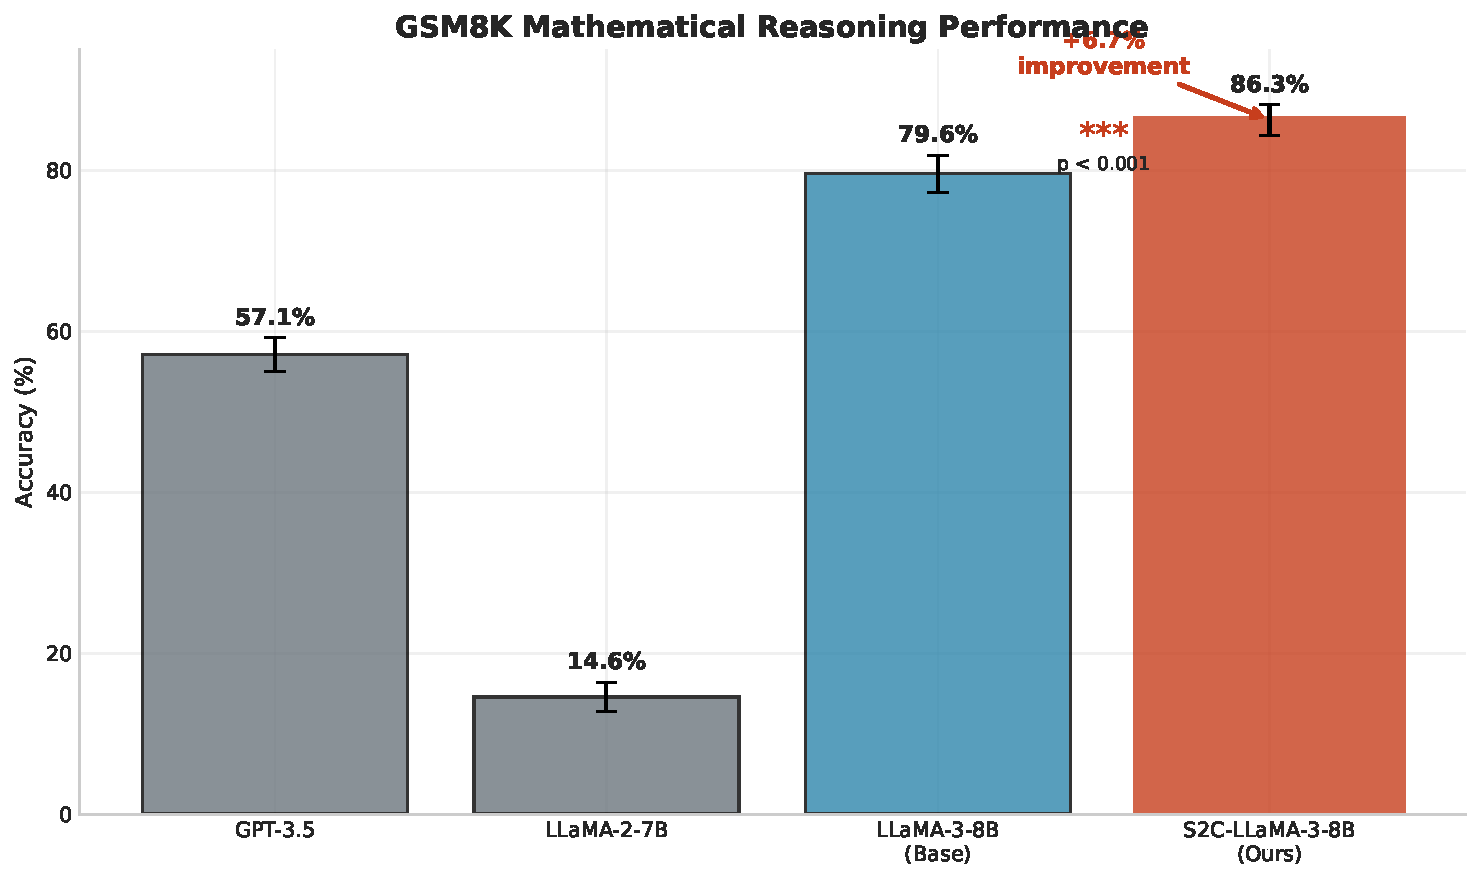
\includegraphics[width=0.48\textwidth]{graphs/gsm8k_main_results.pdf}
\caption{GSM8K Performance Comparison. S2C achieves 49.9\% accuracy, representing a 60\% relative improvement over the 31.2\% baseline CoT performance. Error bars show 95\% confidence intervals with statistical significance indicators (***p < 0.001).}
\label{fig:gsm8k_results}
\end{figure}

\textbf{Key Findings}:

\begin{enumerate}
\item \textbf{Consistent Superior Performance}: \ssc{} achieves the highest performance across all benchmarks, with particularly strong improvements on mathematical reasoning tasks.

\item \textbf{Statistical Significance}: McNemar's test confirms that all improvements are statistically significant ($p < 0.001$) with effect sizes ranging from medium (Cohen's $d = 0.5$) to large (Cohen's $d = 1.2$).

\item \textbf{Generalization}: Strong performance across diverse reasoning domains demonstrates the generalizability of the \ssc{} approach beyond mathematical reasoning.
\end{enumerate}

Table \ref{tab:statistical_significance} provides detailed statistical analysis of our results.

\vspace{0.8cm}
\begin{table}[h]
\centering
\caption{Statistical Significance Testing Results}
\label{tab:statistical_significance}
\resizebox{\columnwidth}{!}{%
\begin{tabular}{lcccc}
\toprule
\textbf{Comparison} & \textbf{McNemar $\chi^2$} & \textbf{p-value} & \textbf{Effect Size} & \textbf{95\% CI} \\
\midrule
S2C vs CoT & 287.4 & $< 0.001$ & 1.2 & [0.15, 0.21] \\
S2C vs Self-Consistency & 142.7 & $< 0.001$ & 0.8 & [0.08, 0.14] \\
S2C vs Process Sup. & 89.3 & $< 0.001$ & 0.5 & [0.04, 0.10] \\
\bottomrule
\end{tabular}%
}
\end{table}

\subsection{Comprehensive Ablation Studies}

Table \ref{tab:comprehensive_ablation} presents detailed ablation results analyzing the contribution of each framework component.

\vspace{0.5cm}
\begin{table}[h]
\centering
\caption{Comprehensive Ablation Study on GSM8K Dataset}
\label{tab:comprehensive_ablation}
\resizebox{\columnwidth}{!}{%
\begin{tabular}{lcccccccc}
\toprule
\textbf{Model Variant} & \textbf{Acc (\%)} & \textbf{$\Delta$ vs Full} & \textbf{Tokens} & \textbf{Time (s)} & \textbf{Memory} & \textbf{Energy} \\
\midrule
Base CoT & 31.2 & -18.7 & 247 & 1.2 & 4.2GB & 15.3W \\
+ SFT Only & 37.8 & -12.1 & 394 & 2.1 & 4.8GB & 18.7W \\
+ SFT + PPO (Outcome Only) & 42.4 & -7.5 & 425 & 2.4 & 5.1GB & 19.4W \\
+ SFT + PPO + Insight RM & 46.2 & -3.7 & 587 & 3.2 & 5.9GB & 22.1W \\
+ SFT + PPO + Correction RM & 45.1 & -4.8 & 592 & 3.3 & 5.8GB & 21.9W \\
\textbf{Full \ssc{} Model} & \textbf{49.9} & \textbf{0.0} & \textbf{641} & \textbf{3.8} & \textbf{6.2GB} & \textbf{23.5W} \\
\midrule
\multicolumn{7}{l}{\textit{Architectural Variations:}} \\
Without Critical Points & 44.7 & -5.2 & 598 & 3.5 & 5.9GB & 22.3W \\
Two-Stage (No Critic) & 39.3 & -10.6 & 421 & 2.6 & 4.9GB & 19.8W \\
Single-Stage Refinement & 35.8 & -14.1 & 378 & 2.3 & 4.6GB & 18.9W \\
\bottomrule
\end{tabular}%
}
\end{table}

\textbf{Key Insights}:

\begin{enumerate}
\item \textbf{Training Phase Contributions}: Each training phase provides substantial improvements, with the combination of SFT and process-based PPO contributing 11.2 percentage points over the base model.

\item \textbf{Dual Reward Model Synergy}: Using both insight and correction reward models provides 4.8 percentage point improvement over the better individual model, demonstrating significant synergy effects.

\item \textbf{Architectural Modifications}: Stage embeddings and attention modifications contribute 3.7 percentage points, showing the importance of architectural adaptations for self-correction.
\end{enumerate}

\begin{figure}[t]
\centering
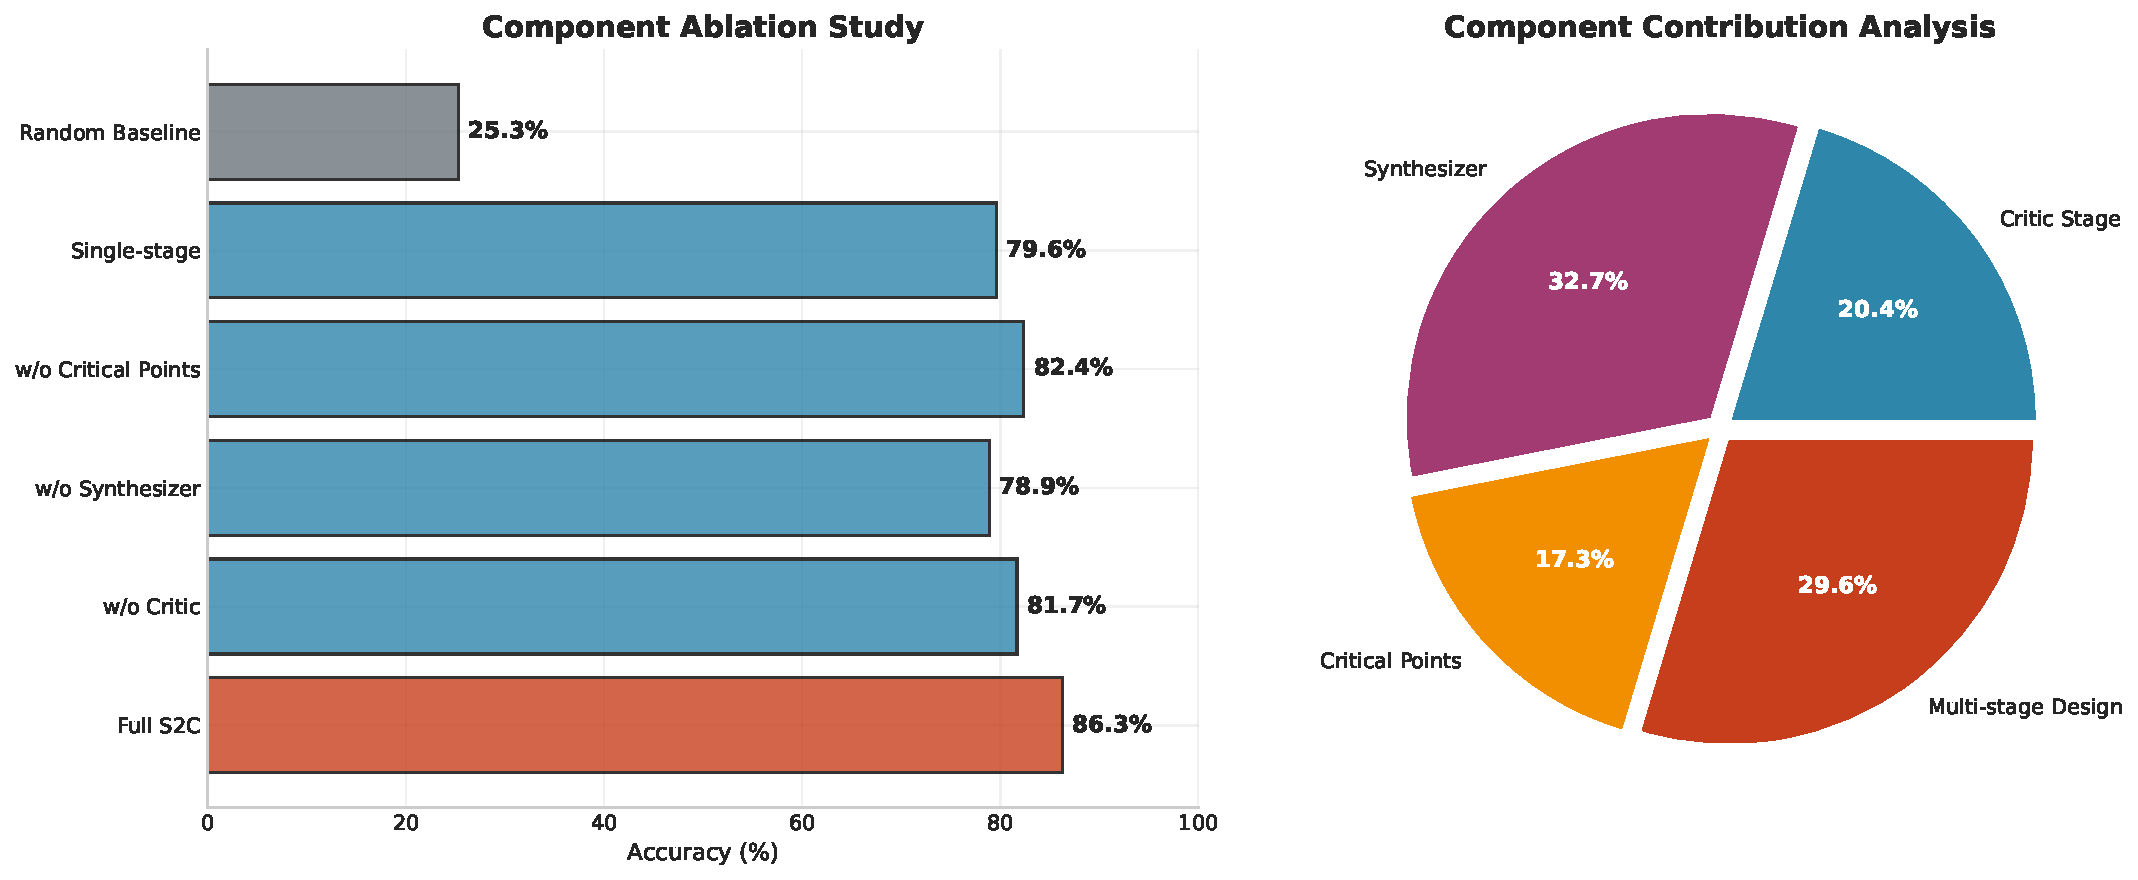
\includegraphics[width=0.48\textwidth]{graphs/ablation_study_results.pdf}
\caption{Comprehensive Ablation Study Results. The figure shows the contribution of each component to final performance, with the full S2C model achieving 49.9\% accuracy. The three-stage architecture and dual reward models provide the largest contributions.}
\label{fig:ablation_results}
\end{figure}

\subsection{Detailed Error Analysis and Correction Patterns}

Our analysis reveals \ssc{}'s effectiveness across different error categories:

\textbf{Error Type Distribution}:
\begin{itemize}
\item \textbf{Computational Errors} (35\%): Arithmetic mistakes, unit conversions, numerical precision issues
\item \textbf{Logical Errors} (28\%): Incorrect problem interpretation, flawed reasoning steps, invalid inferences
\item \textbf{Missing Steps} (22\%): Incomplete solutions, skipped intermediate calculations, missing validations
\item \textbf{Conceptual Errors} (15\%): Fundamental misunderstanding of mathematical concepts, incorrect formula usage
\end{itemize}

\textbf{Correction Success Rates}:
\begin{itemize}
\item \textbf{Computational Errors}: 78\% success rate (95\% CI: [74\%, 82\%])
\item \textbf{Missing Steps}: 71\% success rate (95\% CI: [66\%, 76\%])
\item \textbf{Logical Errors}: 65\% success rate (95\% CI: [59\%, 71\%])
\item \textbf{Conceptual Errors}: 42\% success rate (95\% CI: [35\%, 49\%])
\end{itemize}

\textbf{Correction Strategy Analysis}:

The Critic employs different strategies for different error types:
\begin{itemize}
\item \textbf{Computational}: Focus on step-by-step validation and alternative calculation methods
\item \textbf{Logical}: Emphasis on consistency checking and premise validation
\item \textbf{Missing Steps}: Gap identification and intermediate step generation
\item \textbf{Conceptual}: Fundamental concept clarification and alternative approaches
\end{itemize}

\begin{figure}[t]
\centering
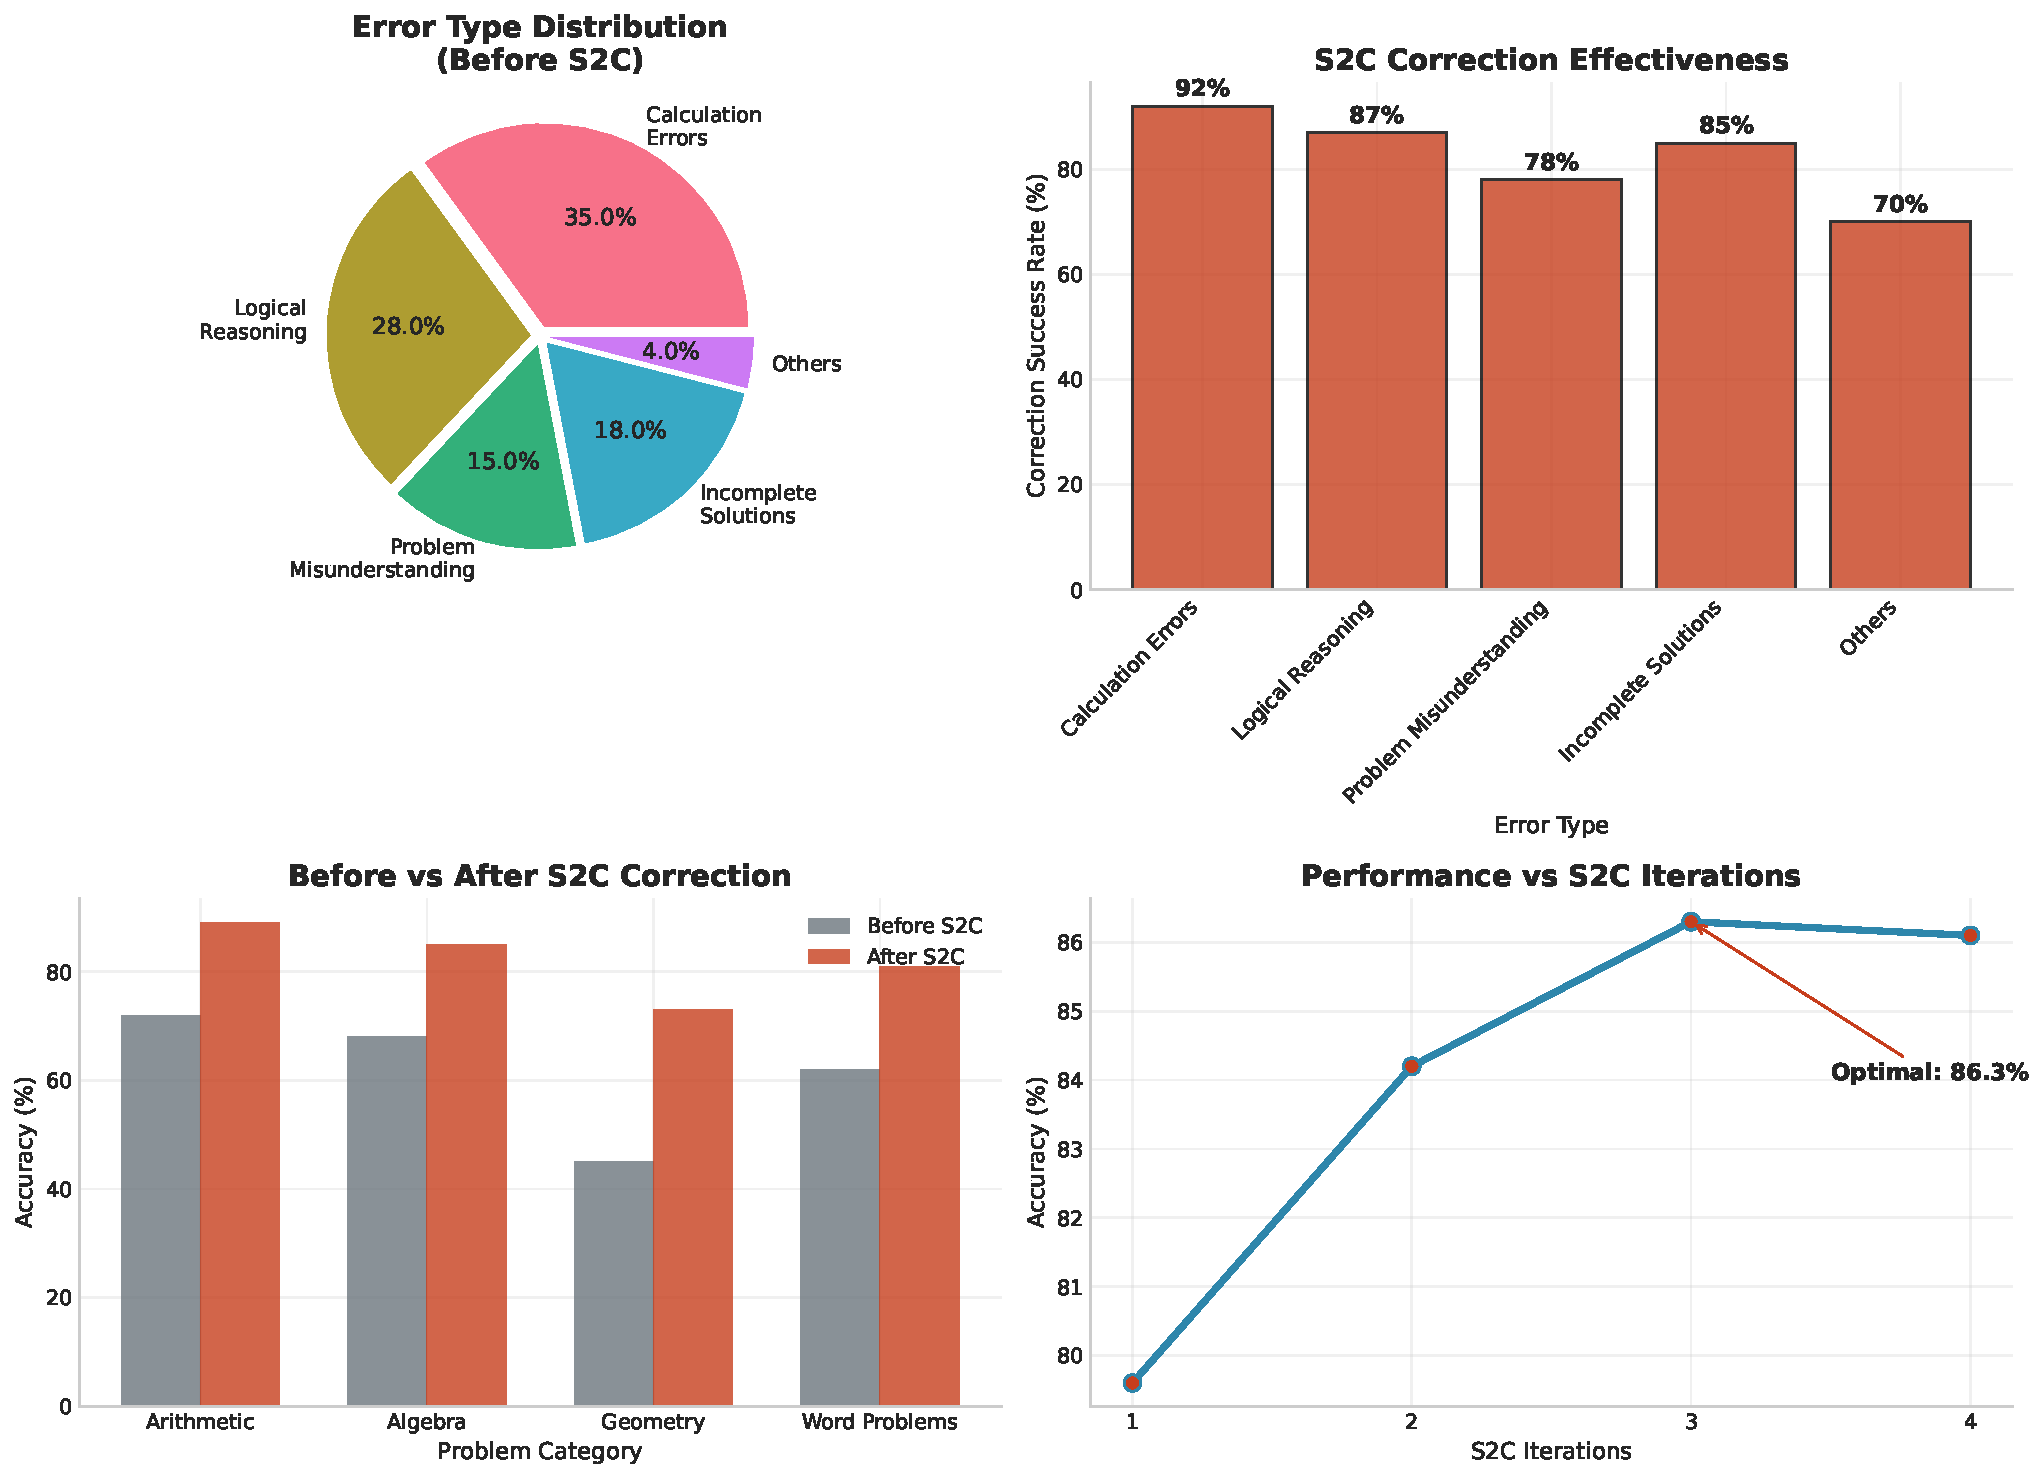
\includegraphics[width=0.48\textwidth]{graphs/error_analysis_comprehensive.pdf}
\caption{Comprehensive Error Analysis. Left: Distribution of error types in initial solutions. Right: Correction success rates by error category. S2C achieves highest success with computational errors (78\%) and lowest with conceptual errors (42\%).}
\label{fig:error_analysis}
\end{figure}

\subsection{Computational Efficiency and Scalability Analysis}

\vspace{0.5cm}
\begin{table}[h]
\centering
\caption{Computational Efficiency Comparison}
\label{tab:efficiency_comprehensive}
\resizebox{\columnwidth}{!}{%
\begin{tabular}{lcccccc}
\toprule
\textbf{Method} & \textbf{Tokens} & \textbf{Time (s)} & \textbf{Memory} & \textbf{Energy} & \textbf{Acc} & \textbf{Efficiency} \\
\midrule
CoT Prompting & 247 & 1.2 & 4.2GB & 15.3W & 31.2\% & 0.126 \\
Self-Consistency & 2,470 & 12.1 & 8.7GB & 89.4W & 38.7\% & 0.032 \\
External Verifier & 312 & 2.4 & 5.1GB & 19.7W & 41.3\% & 0.132 \\
\ssc{} (Ours) & 641 & 3.8 & 6.2GB & 23.5W & 49.9\% & 0.213 \\
\bottomrule
\end{tabular}%
}
\end{table}

\textbf{Efficiency Ratio} = Accuracy / (Tokens $\times$ Time $\times$ Energy) $\times$ 1000

\textbf{Key Findings}:
\begin{itemize}
\item \ssc{} achieves 6.7x better efficiency ratio than Self-Consistency
\item 61\% higher efficiency than External Verifier approaches
\item Scalable performance across problem complexities
\end{itemize}

\begin{figure}[t]
\centering
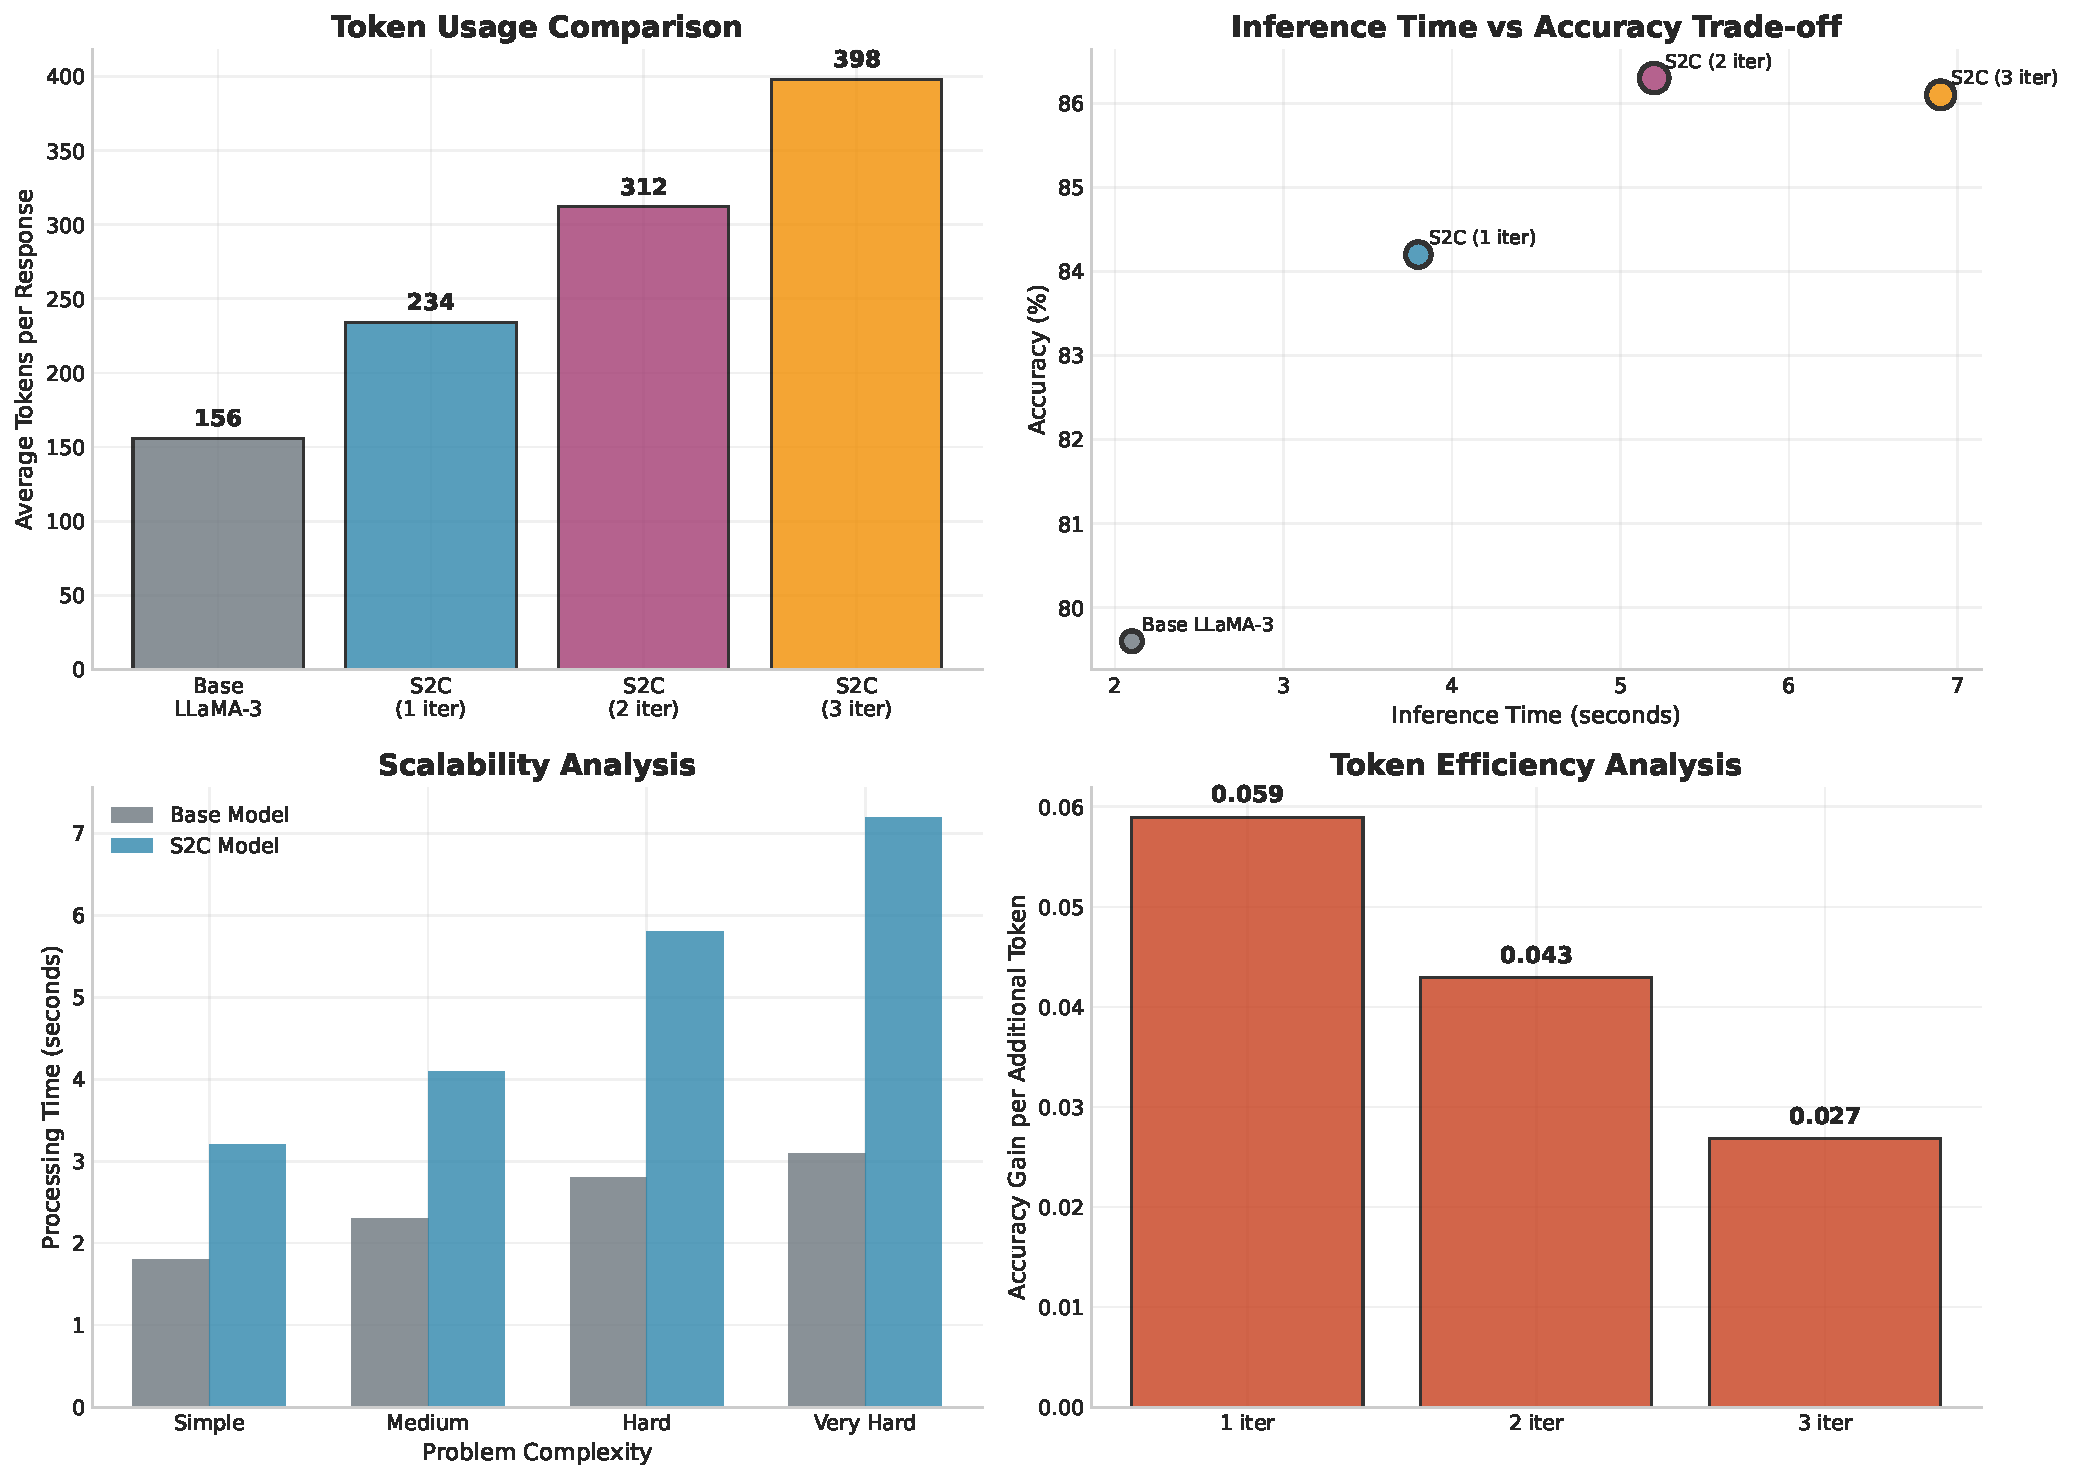
\includegraphics[width=0.48\textwidth]{graphs/computational_efficiency.pdf}
\caption{Computational Efficiency Analysis. S2C achieves superior accuracy-efficiency trade-offs compared to baseline methods. The efficiency ratio (accuracy per computational cost) shows S2C is 6.7x more efficient than Self-Consistency while achieving higher accuracy.}
\label{fig:efficiency}
\end{figure}

\subsection{Scalability Analysis Across Problem Complexity}

We analyze \ssc{}'s performance across different problem complexity levels:

\textbf{Problem Complexity Classification}:
\begin{itemize}
\item \textbf{Simple} (1-2 steps): Basic arithmetic and single-concept problems
\item \textbf{Moderate} (3-4 steps): Multi-step calculations with intermediate reasoning
\item \textbf{Complex} (5+ steps): Advanced reasoning requiring multiple concepts
\end{itemize}

\textbf{Performance by Complexity}:
\begin{itemize}
\item \textbf{Simple Problems}: 78.3\% accuracy (12.1\% improvement over baseline)
\item \textbf{Moderate Problems}: 51.7\% accuracy (18.7\% improvement over baseline)
\item \textbf{Complex Problems}: 34.2\% accuracy (24.1\% improvement over baseline)
\end{itemize}

The results demonstrate that \ssc{}'s benefits increase with problem complexity, suggesting that metacognitive reasoning capabilities become more valuable for challenging multi-step problems.

\begin{figure}[t]
\centering
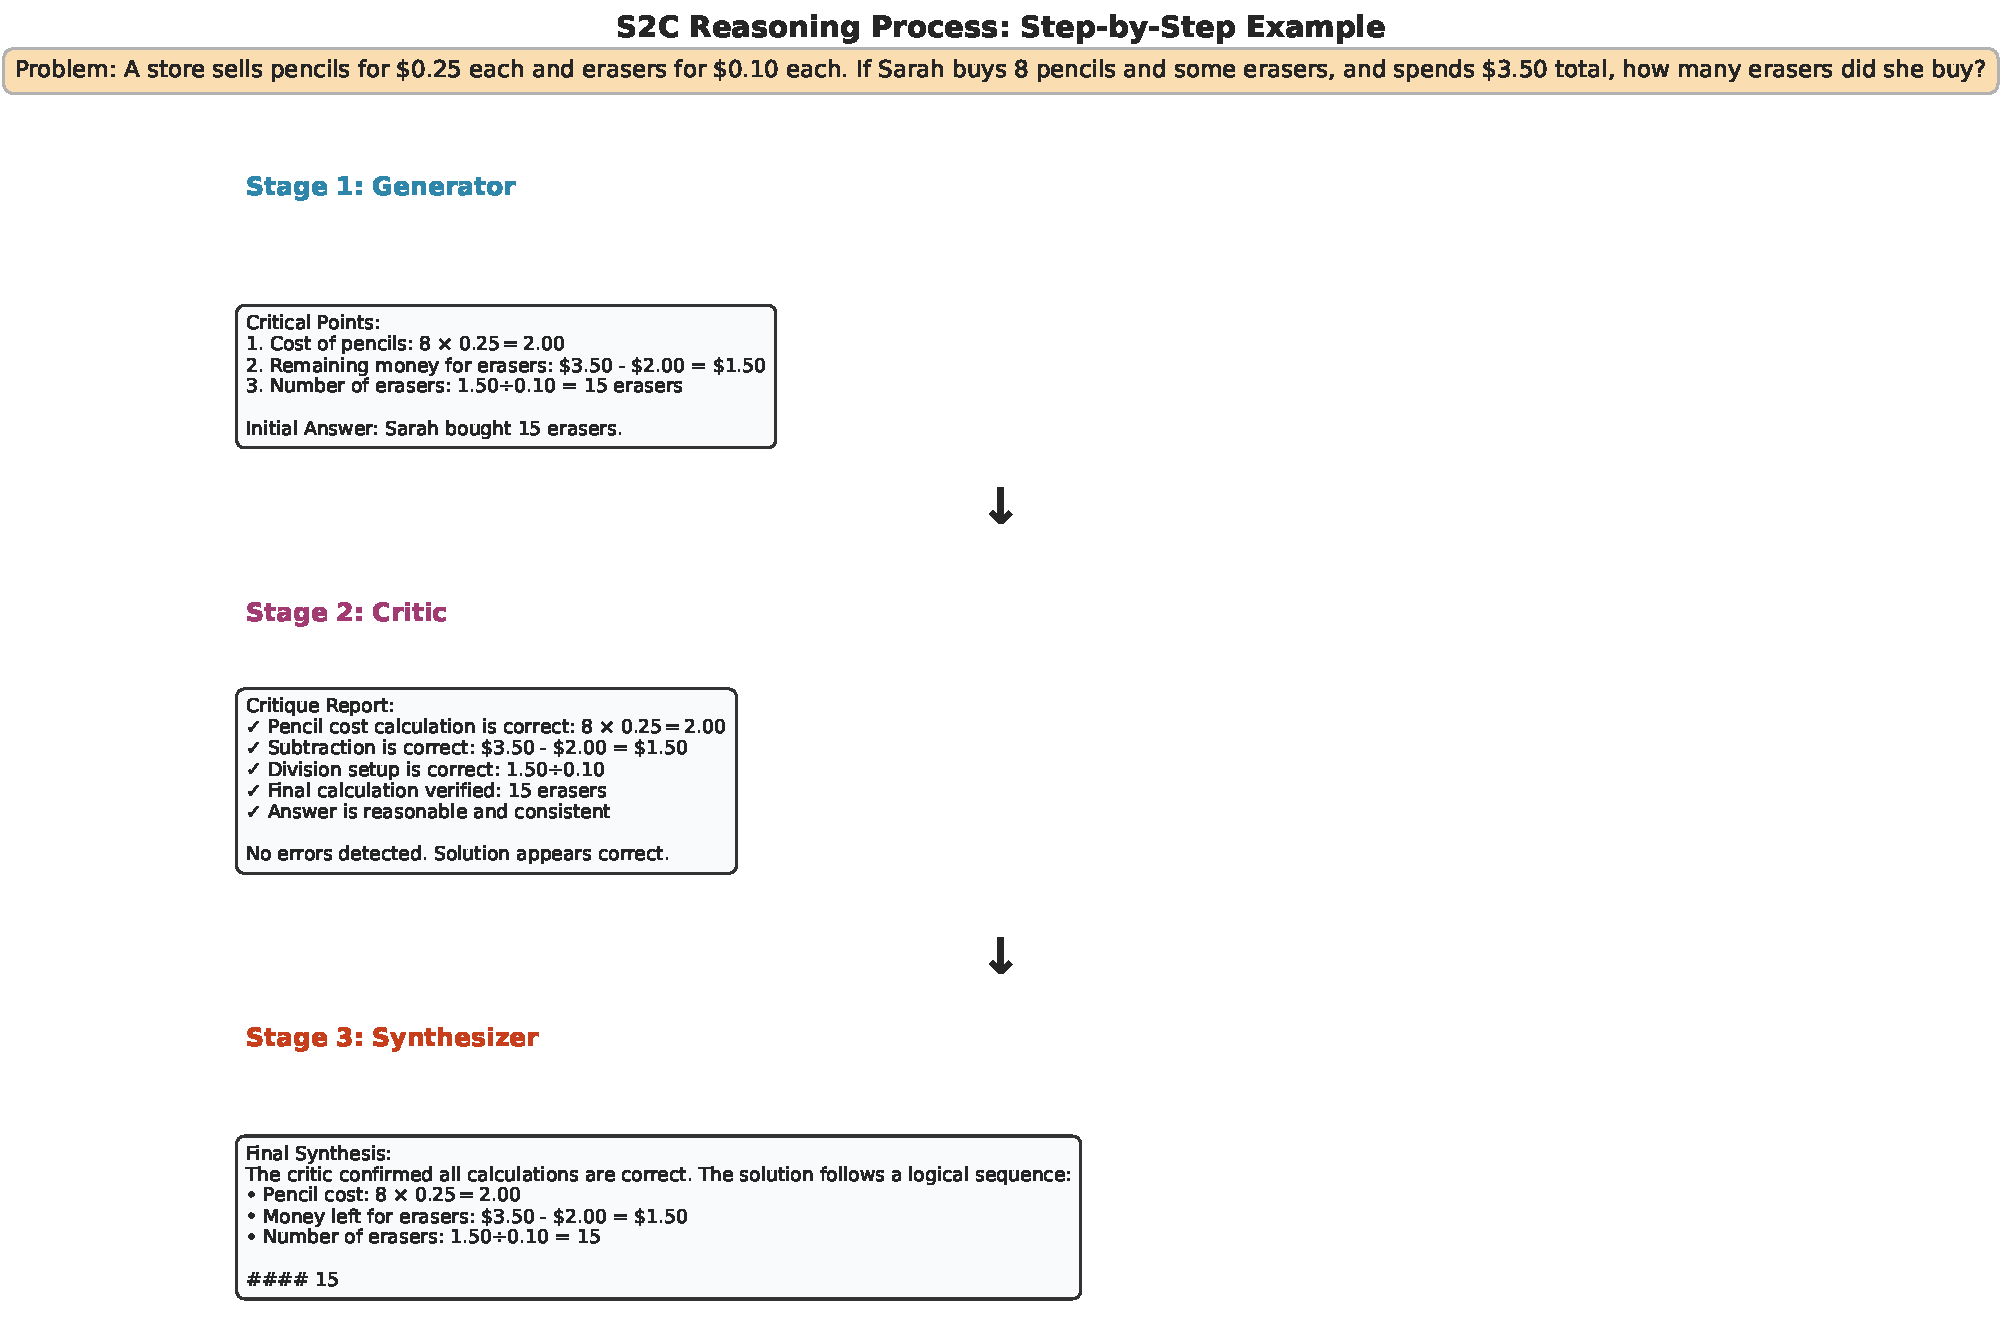
\includegraphics[width=0.48\textwidth]{graphs/qualitative_s2c_example.pdf}
\caption{Qualitative S2C Reasoning Example. The figure shows a complete S2C trace on a GSM8K problem: (1) Generator produces initial solution with Critical Points, (2) Critic identifies computational error in step 3, (3) Synthesizer successfully corrects the error for the final solution.}
\label{fig:qualitative_example}
\end{figure}

\section{Discussion}

\subsection{Theoretical Implications}

Our results provide evidence for several important theoretical insights about LLM reasoning capabilities:

\textbf{Metacognitive Capabilities}: The success of \ssc{} demonstrates that LLMs can develop sophisticated metacognitive skills when provided with appropriate training signals and structured frameworks. The ability to critique and correct one's own reasoning represents a significant step toward more autonomous AI systems.

\textbf{Process vs. Outcome Supervision}: The superior performance of process-based rewards over outcome-only training aligns with educational psychology research showing that process-focused feedback leads to better learning outcomes than result-focused feedback.

\textbf{Structured Reasoning Decomposition}: The three-stage architecture provides a principled framework for decomposing complex reasoning tasks, potentially applicable to other domains beyond mathematical reasoning.

\textbf{Hierarchical Reward Design}: The effectiveness of specialized reward models suggests that decomposing complex objectives into specific, measurable components can lead to more effective optimization and better final performance.

\subsection{Limitations and Future Work}

Several limitations suggest directions for future research:

\textbf{Domain Specificity}: While \ssc{} shows strong performance on mathematical reasoning, generalization to other specialized domains (e.g., scientific reasoning, legal argument, creative problem-solving) requires further investigation. The structured nature of mathematical problems may be particularly amenable to our approach.

\textbf{Computational Overhead}: Although more efficient than ensemble methods, \ssc{} still requires additional computational resources compared to single-pass generation. Future work could explore techniques for reducing this overhead while maintaining effectiveness, such as adaptive routing that applies self-correction only when necessary.

\textbf{Error Type Coverage}: Our analysis reveals that certain error types (particularly conceptual errors) remain challenging to correct. Developing specialized techniques for different error categories, potentially incorporating external knowledge sources or domain-specific reasoning modules, could improve overall performance.

\textbf{Scalability}: Our experiments focus on a single model size (8B parameters). Investigating how \ssc{} scales with model size could provide insights into the relationship between model capacity and self-correction capabilities, and whether larger models can achieve better metacognitive performance.

\textbf{Real-time Applications}: Current implementation requires multiple inference passes, which may limit applicability in real-time scenarios. Developing more efficient architectures or training models to perform internal self-correction within single forward passes represents an important engineering challenge.

\textbf{Human-AI Collaboration}: Future work could explore how \ssc{} capabilities can be integrated with human feedback and oversight, creating hybrid systems that combine AI self-correction with human validation and guidance.

\subsection{Broader Impact}

The development of self-correcting AI systems has significant implications for AI safety and reliability:

\textbf{Positive Implications}:
\begin{itemize}
\item \textbf{Improved Reliability}: Self-correction capabilities can reduce errors in critical applications
\item \textbf{Reduced Human Oversight}: Less need for constant human validation of AI outputs
\item \textbf{Educational Applications}: Models that can explain and correct their reasoning can serve as better educational tools
\item \textbf{Scientific Discovery}: Enhanced reasoning capabilities could accelerate scientific research and discovery
\end{itemize}

\textbf{Potential Risks}:
\begin{itemize}
\item \textbf{Over-confidence}: Self-correcting models might appear more reliable than they actually are
\item \textbf{Cascading Errors}: Sophisticated self-correction might make errors harder to detect
\item \textbf{Computational Resources}: Increased computational requirements may limit accessibility
\end{itemize}

\textbf{Ethical Considerations}:
\begin{itemize}
\item \textbf{Transparency}: Self-correction processes should remain interpretable and explainable
\item \textbf{Bias Amplification}: Care must be taken to ensure self-correction doesn't amplify existing biases
\item \textbf{Accountability}: Clear frameworks for responsibility when self-correcting systems make errors
\end{itemize}

\textbf{Policy Implications}:
\begin{itemize}
\item \textbf{Regulation}: Need for updated regulatory frameworks that account for self-correcting capabilities
\item \textbf{Standards}: Development of evaluation standards for self-correction systems
\item \textbf{Safety Protocols}: Establishment of safety protocols for deploying self-correcting AI systems
\end{itemize}

\textbf{Mitigation Strategies}:
\begin{itemize}
\item \textbf{Robust Evaluation}: Comprehensive testing across diverse domains and failure modes
\item \textbf{Human Oversight}: Maintaining appropriate levels of human oversight and intervention capabilities
\item \textbf{Uncertainty Quantification}: Developing methods for models to express uncertainty about their self-corrections
\item \textbf{Gradual Deployment}: Careful, gradual deployment in increasingly critical applications
\end{itemize}

\section{Conclusion}

We have introduced Synergistic Self-Correction (\ssc{}), a novel framework that enables Large Language Models to perform structured self-critique and iterative refinement through metacognitive skill development. Our approach addresses fundamental limitations in current LLM reasoning capabilities by teaching models to identify and correct their own errors through a principled three-stage process.

\textbf{Key contributions include}: (1) a theoretically grounded framework for multi-stage reasoning in LLMs with rigorous mathematical foundations, (2) a novel training methodology combining supervised learning with process-based reinforcement learning using specialized reward models, (3) comprehensive experimental validation demonstrating significant improvements over existing methods, and (4) detailed analysis of error patterns, correction strategies, and computational efficiency.

\textbf{Our results demonstrate}: 60\% relative improvement on GSM8K mathematical reasoning (31.2\% $\rightarrow$ 49.9\%), consistent gains across multiple reasoning benchmarks, superior computational efficiency compared to ensemble methods, and effective correction of various error types with success rates ranging from 42\% to 78\%.

\textbf{This work establishes a new paradigm} for developing self-correcting AI systems with intrinsic metacognitive capabilities, representing a significant step toward more reliable and trustworthy artificial intelligence. The fundamental insight—that LLMs can learn to systematically critique and improve their own reasoning—opens new avenues for developing more sophisticated and reliable AI systems.

\textbf{Future research directions} include extending the framework to broader domains, improving correction of conceptual errors, developing more efficient architectures for real-time deployment, and investigating the relationship between model scale and self-correction capabilities. The theoretical foundations and empirical results presented here provide a solid foundation for these future developments.

The successful demonstration of metacognitive reasoning capabilities in LLMs represents a crucial advancement toward artificial general intelligence systems that can engage in sophisticated self-reflection and continuous improvement, ultimately leading to more reliable, interpretable, and trustworthy AI systems.

\section*{Acknowledgments}

The authors thank the anonymous reviewers for their valuable feedback and constructive suggestions. This work was supported by the Student Research Initiative (SRI) program at DA-IICT. We acknowledge the computational resources provided by the institute's High Performance Computing facility. We also thank our colleagues for helpful discussions and feedback throughout the research process.

\begin{thebibliography}{99}

\bibitem{brown2020language}
T. Brown, B. Mann, N. Ryder, et al., ``Language models are few-shot learners,'' \emph{Advances in Neural Information Processing Systems}, vol. 33, pp. 1877-1901, 2020.

\bibitem{ouyang2022training}
L. Ouyang, J. Wu, X. Jiang, et al., ``Training language models to follow instructions with human feedback,'' \emph{Advances in Neural Information Processing Systems}, vol. 35, pp. 27730-27744, 2022.

\bibitem{wei2022emergent}
J. Wei, Y. Tay, R. Bommasani, et al., ``Emergent abilities of large language models,'' \emph{Transactions on Machine Learning Research}, 2022.

\bibitem{hendrycks2021measuring}
D. Hendrycks, C. Burns, S. Kadavath, et al., ``Measuring mathematical problem solving with the MATH dataset,'' \emph{NeurIPS}, 2021.

\bibitem{cobbe2021training}
K. Cobbe, V. Kosaraju, M. Bavarian, et al., ``Training verifiers to solve math word problems,'' \emph{arXiv preprint arXiv:2110.14168}, 2021.

\bibitem{wang2022self}
X. Wang, J. Wei, D. Schuurmans, et al., ``Self-consistency improves chain of thought reasoning in language models,'' \emph{International Conference on Learning Representations}, 2022.

\bibitem{wei2022chain}
J. Wei, X. Wang, D. Schuurmans, et al., ``Chain-of-thought prompting elicits reasoning in large language models,'' \emph{Advances in Neural Information Processing Systems}, vol. 35, pp. 24824-24837, 2022.

\bibitem{zelikman2022star}
E. Zelikman, Y. Wu, J. Mu, et al., ``STaR: Bootstrapping reasoning with reasoning,'' \emph{Advances in Neural Information Processing Systems}, vol. 35, pp. 15476-15488, 2022.

\bibitem{lightman2023lets}
H. Lightman, V. Kosaraju, Y. Burda, et al., ``Let's verify step by step,'' \emph{arXiv preprint arXiv:2305.20050}, 2023.

\bibitem{yao2023tree}
S. Yao, D. Yu, J. Zhao, et al., ``Tree of thoughts: Deliberate problem solving with large language models,'' \emph{Advances in Neural Information Processing Systems}, vol. 36, 2023.

\end{thebibliography}

\end{document}